\documentclass[a4paper,12pt,twoside]{book}

\usepackage{graphicx}

%For captions 
\usepackage[labelfont=bf,justification=centering]{caption}
\usepackage[font=small,labelfont=bf]{subcaption}
\captionsetup[sub]{font=tiny,labelfont={bf,sf}}

\usepackage{booktabs}
\usepackage{float}
\usepackage[flushleft]{threeparttable}

\begin{document}
dtbn

\begin{table}[H]
	\centering
	\fontsize{8}{10}\selectfont
	\begin{tabular}{llllll}
		\hline		Variable & Group & Top 20 & Middle 40 & Bottom 20 & Whole Sample \\ 
		\hline
		edu\_yrs & Female older & 13.38 (2.62) & 13.91 (2.73) & 13.91 (2.7) & 13.76 (2.71) \\ 
		&Female young & 14.09 (2.75) & 14.55 (2.66) & 14.8 (2.61) & 14.49 (2.68) \\ 
		&Male older & 12.51 (2.34) & 13.21 (2.66) & 13.26 (2.68) & 13.03 (2.6) \\ 
		&Male young & 13.04 (2.58) & 13.83 (2.74) & 14.02 (2.75) & 13.67 (2.73) \\ 
		wage & Female older & 19379.02 (11665.53) & 27784.51 (18811.94) & 26329.79 (16935.15) & 25132.36 (17104.73) \\ 
		&Female young & 19731.68 (10639.46) & 30433.91 (20443.96) & 27890.92 (16672.82) & 27170.08 (18149.23) \\ 
		&Male older & 26392.05 (18023.65) & 36872.17 (26937.81) & 35302.24 (24426.05) & 33650.33 (24684.13) \\ 
		&Male young & 31539.2 (18744.09) & 40202.54 (24260.45) & 37103.45 (24277.62) & 37266.07 (23242.51) \\
		\midrule
		Priority regions &  & \begin{tabular}[l]{@{}l@{}}Pskovskaya Obl.,\\ Resp. Karelia, \\Resp. Mariy El\end{tabular} & \begin{tabular}[l]{@{}l@{}}Altayskiy Kray, \\Kurganskaya Obl.,\\ Chuvashskaya Resp.,\\ Resp.a Altay \end{tabular}& \begin{tabular}[l]{@{}l@{}}Resp. Adygeya,\\ Resp. Kalmykiya,\\ Resp. Tyva \end{tabular}& \begin{tabular}[l]{@{}l@{}} Resp. Adygeya,\\ Pskovskaya Obl.,\\ Altayskiy Kray,\\ Kurganskaya Obl.,\\ Resp. Kalmykiya, \\ Chuvashskaya Resp.,\\ Res. Altay,\\ Resp. Karelia,\\ Resp. Tyva,\\ Resp. Mariy El \end{tabular}\\ 
		\hline
	\end{tabular}
    \begin{tablenotes}
	\small
	\item This is where authors provide additional information about
	the data, including whatever notes are needed.
\end{tablenotes}
\end{table}


\begin{table}[ht]
	\centering
	\begin{tabular}{rllllll}
		\hline
		Variable & Group & Top 20 & Middle 40 & Bottom 20 & Whole Sample \\ 
		\hline
		edu\_yrs & Female older & 13.38 (2.62) & 13.91 (2.73) & 13.91 (2.7) & 13.76 (2.71) \\ 
		Female young & 14.09 (2.75) & 14.55 (2.66) & 14.8 (2.61) & 14.49 (2.68) \\ 
		Male older & 12.51 (2.34) & 13.21 (2.66) & 13.26 (2.68) & 13.03 (2.6) \\ 
		Male young & 13.04 (2.58) & 13.83 (2.74) & 14.02 (2.75) & 13.67 (2.73) \\ 
		wage & Female older & 19379.02 (11665.53) & 27784.51 (18811.94) & 26329.79 (16935.15) & 25132.36 (17104.73) \\ 
		Female young & 19731.68 (10639.46) & 30433.91 (20443.96) & 27890.92 (16672.82) & 27170.08 (18149.23) \\ 
		Male older & 26392.05 (18023.65) & 36872.17 (26937.81) & 35302.24 (24426.05) & 33650.33 (24684.13) \\ 
		Male young & 31539.2 (18744.09) & 40202.54 (24260.45) & 37103.45 (24277.62) & 37266.07 (23242.51) \\ 
		Priority regions &  & Pskovskaya Oblast, Respublika Karelia, Respublika Mariy El & Altayskiy Kray, Kurganskaya Oblast, Chuvashskaya Respublika, Respublika Altay & Respublika Adygeya, Respublika Kalmykiya, Respublika Tyva & Respublika Adygeya, Pskovskaya Oblast, Altayskiy Kray, Kurganskaya Oblast, Respublika Kalmykiya, Chuvashskaya Respublika, Respublika Altay, Respublika Karelia, Respublika Tyva, Respublika Mariy El \\ 
		\hline
	\end{tabular}
\end{table}

\begin{table}[ht]
	\centering
	\begin{tabular}{llrlrlrlr}
		\hline
		IVs & Female\_young & N1 & Female\_old & N2 & Male\_young & N3 & Male\_old & N4 \\ 
		\hline
		high\_n & 1.959 (0.229) & 9779 & 0.857 (0.042) & 11564 & 0.787 (0.047) & 10636 & 0.64 (0.026) & 9826 \\ 
		HSGPER & 1.717 (0.174) & 9779 & 0.887 (0.044) & 11564 & 0.754 (0.043) & 10636 & 0.636 (0.026) & 9826 \\ 
		s1z & 1.34 (0.195) & 9779 & 0.602 (0.041) & 11564 & 0.648 (0.06) & 10636 & 0.501 (0.034) & 9826 \\ 
		migrationrate & 1.429 (0.163) & 9779 & 0.796 (0.05) & 11564 & 0.625 (0.045) & 10636 & 0.534 (0.028) & 9826 \\ 
		women2menratio & -0.439 (0.609) & 9779 & -0.99 (0.731) & 11564 & -0.105 (0.154) & 10636 & -2.998 (5.602) & 9826 \\ 
		marriagerate & 2.312 (0.536) & 9779 & 2.18 (0.477) & 11564 & 2.638 (0.705) & 10636 & 1.988 (0.378) & 9826 \\ 
		fem\_ind\_prop & 1.677 (0.218) & 9779 & 0.985 (0.079) & 11564 & 0.829 (0.066) & 10636 & 0.663 (0.034) & 9826 \\ 
		Literacy\_97 & 1.868 (0.232) & 6834 & 0.912 (0.053) & 7860 & 0.726 (0.044) & 7247 & 0.641 (0.03) & 6701 \\ 
		OLS & 0.092 (0.003) & 9775 & 0.107 (0.003) & 11560 & 0.103 (0.003) & 10632 & 0.114 (0.003) & 9822 \\ 
		\hline
	\end{tabular}
\end{table}


	
\begin{figure}[htbp!]
	\begin{minipage}[b]{\textwidth}
		\centering
		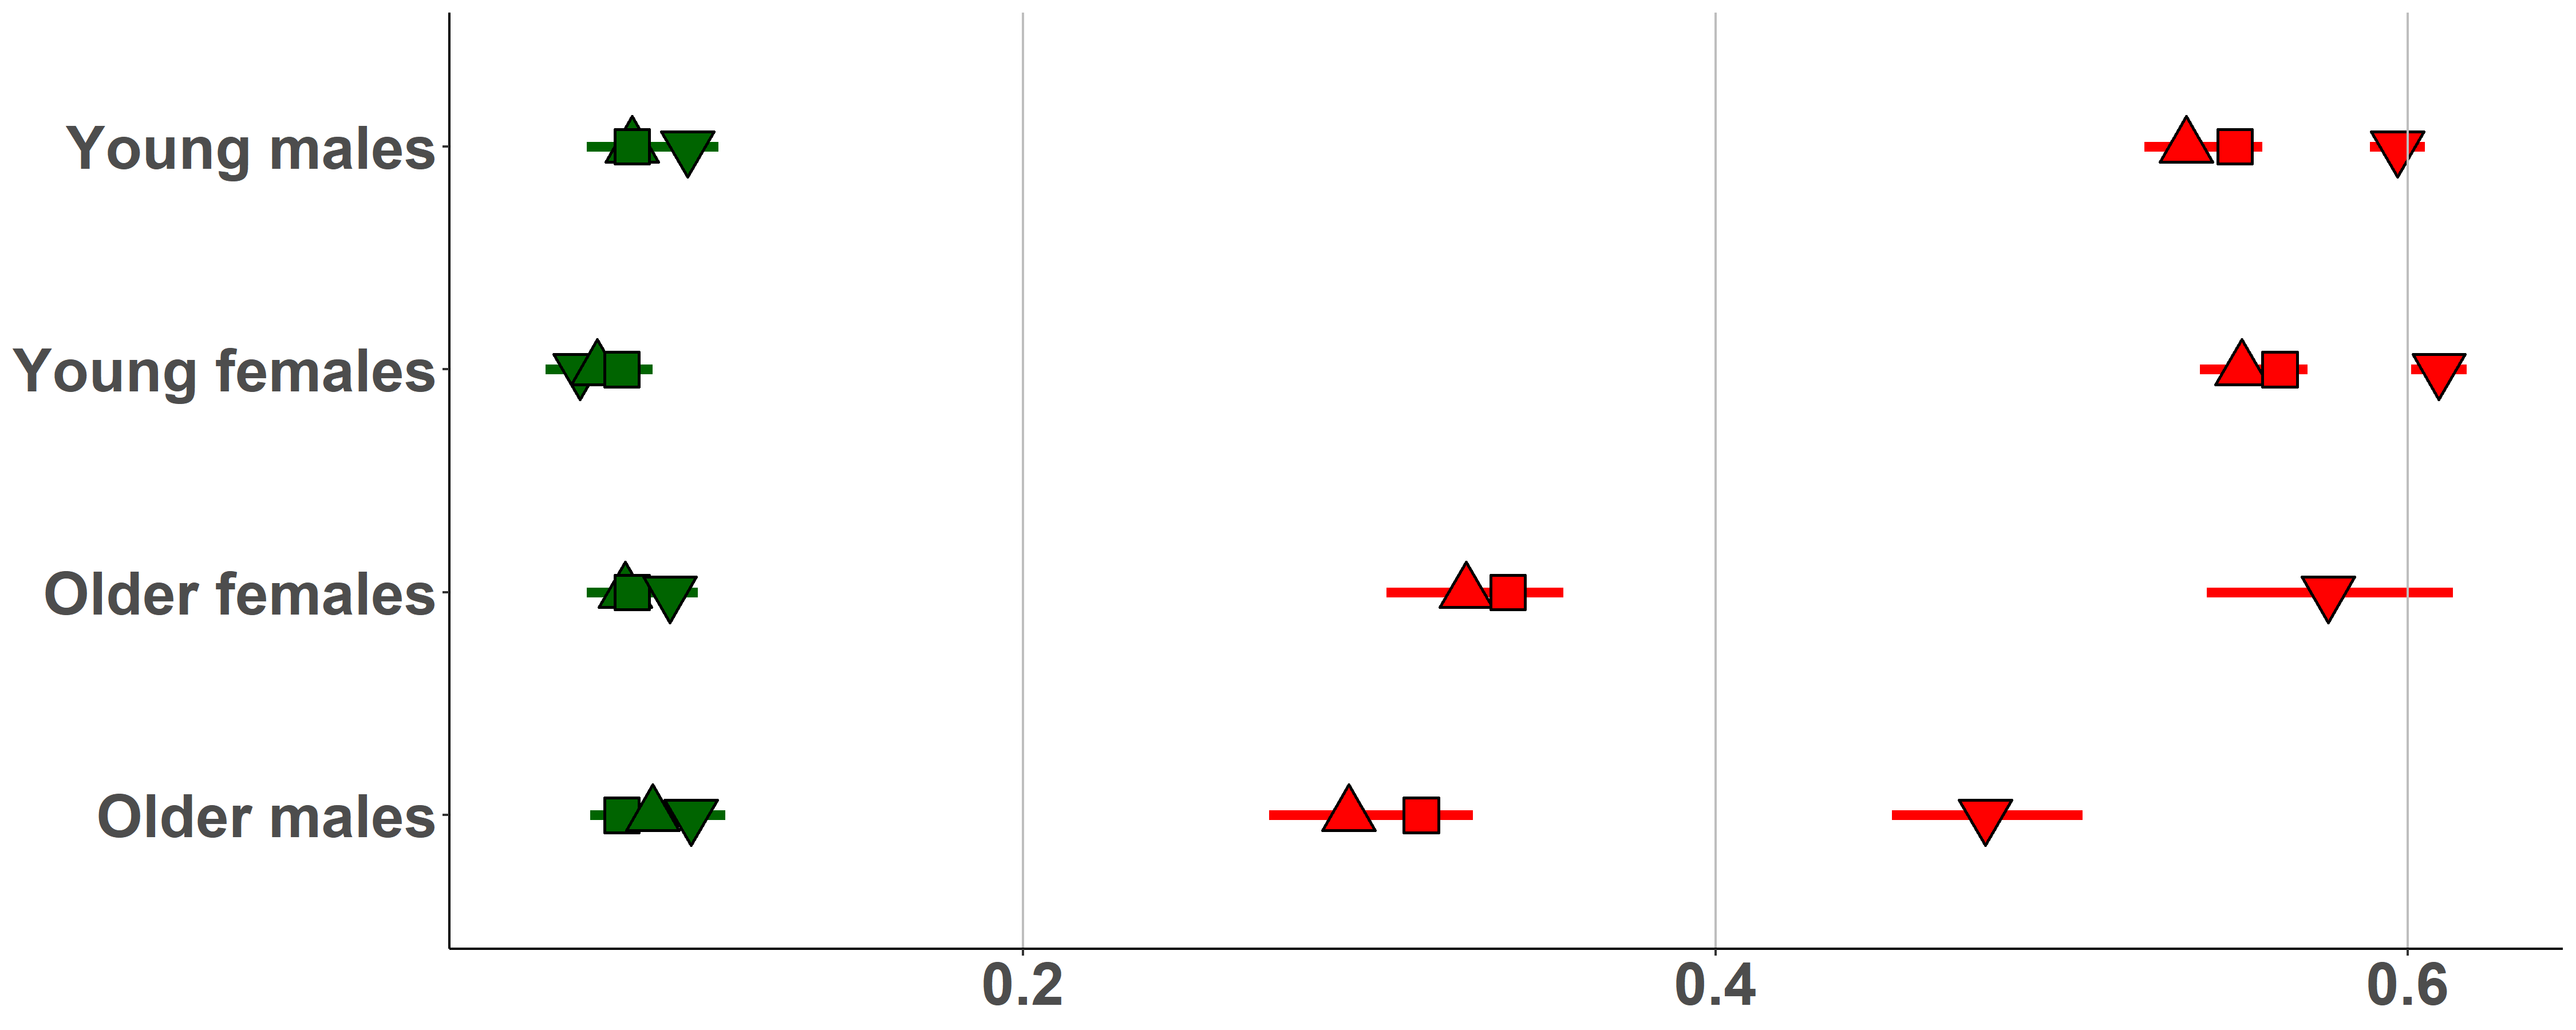
\includegraphics[width=\textwidth]{iv_2_methods_1.png}
		\subcaption{Ranking variable: \\
			regional percentage of \\
			vocational education as final level amongst women 25-64}\label{fig:5.4a}
	\end{minipage}
	\hfill
	\begin{minipage}[b]{\textwidth}
		\centering
		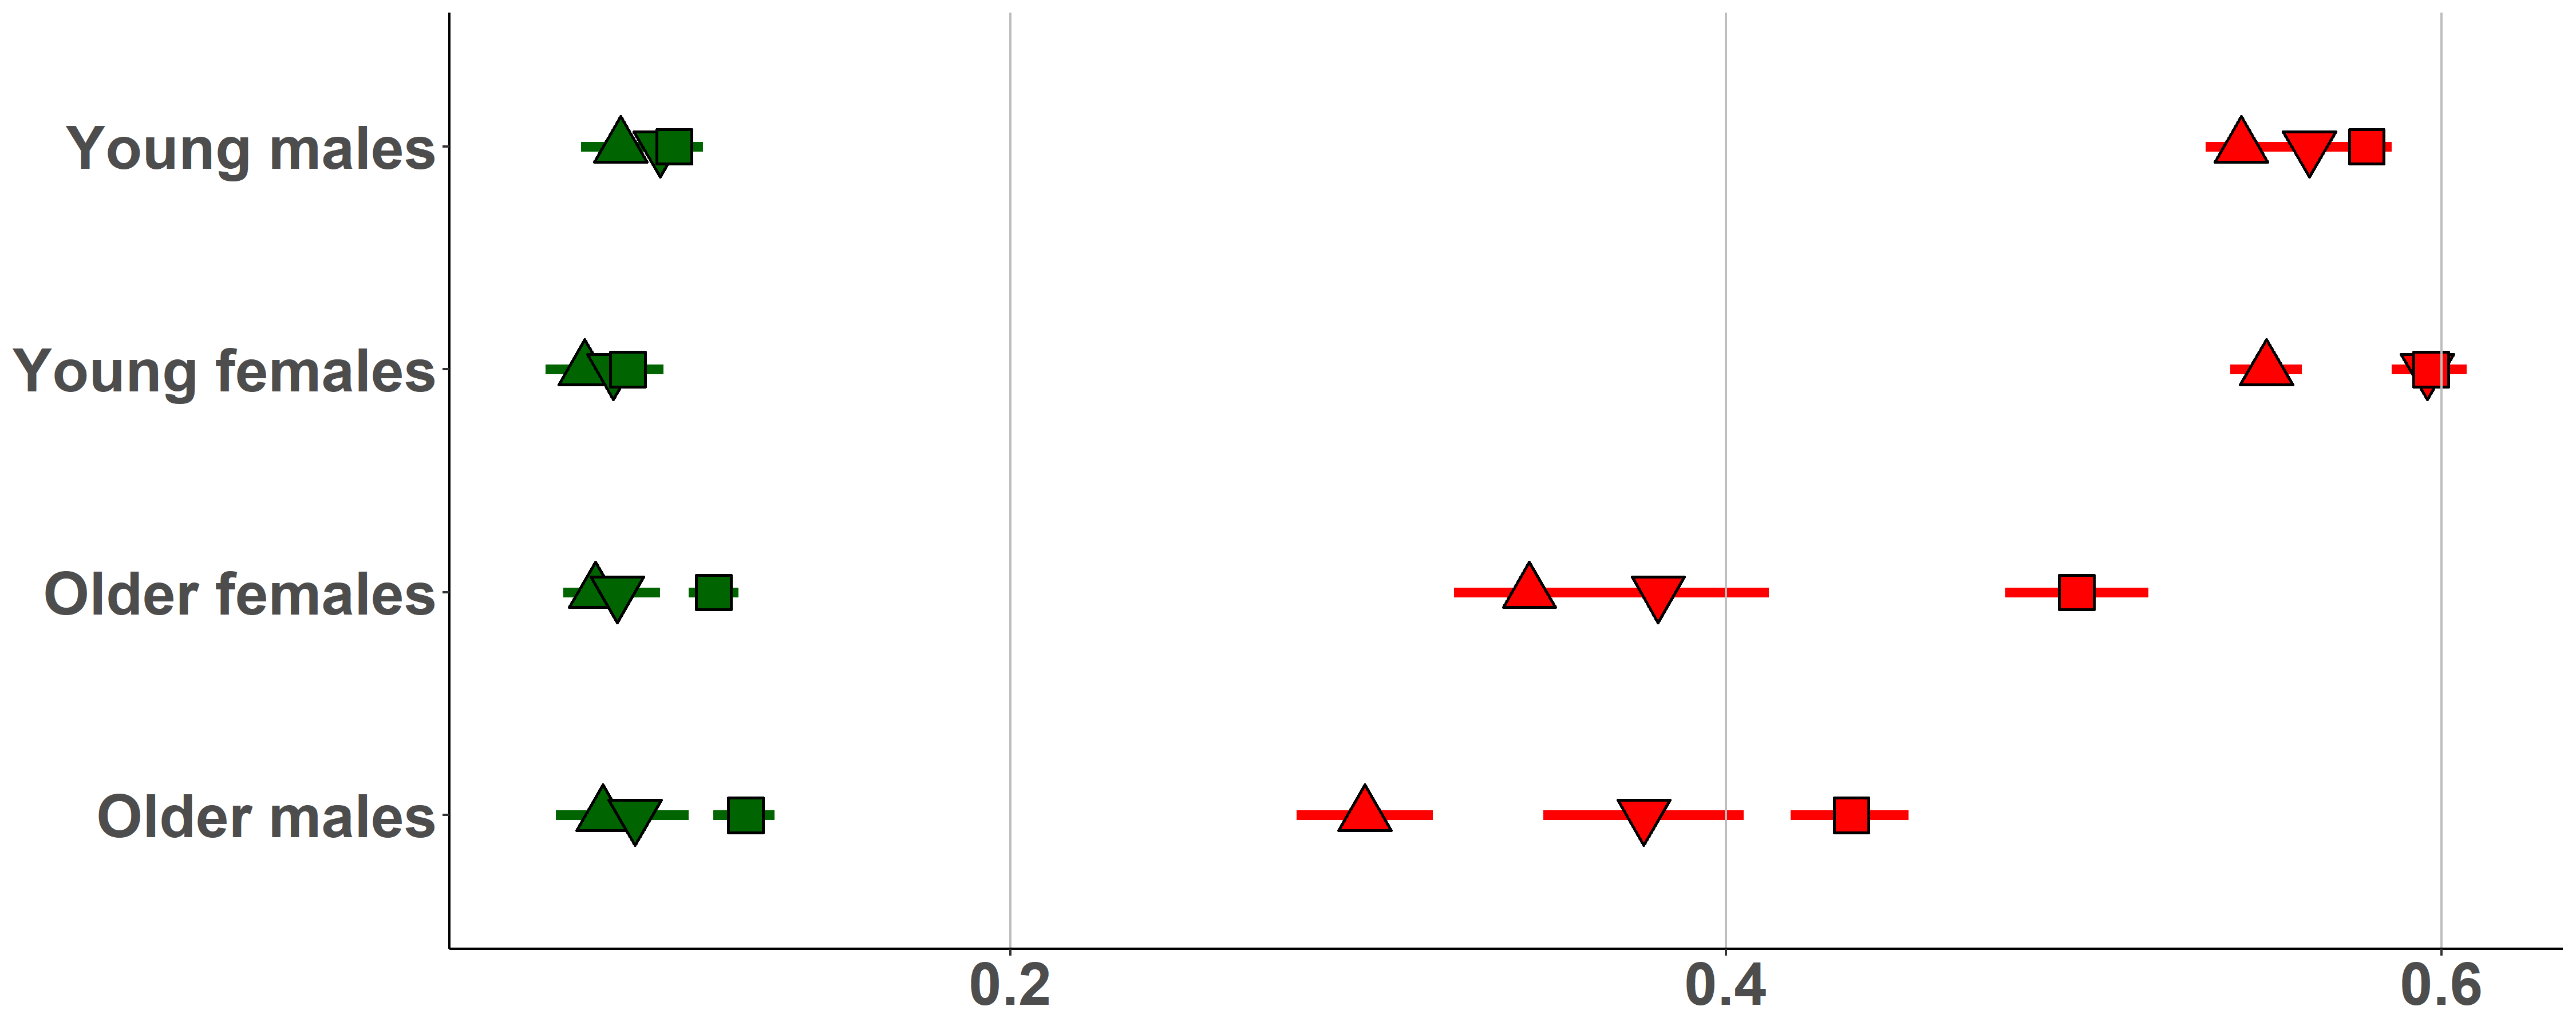
\includegraphics[width=\textwidth]{iv_2_methods_2.png}
		\subcaption{Ranking variable: regional level of employment among vocational level holders}\label{fig:5.4b}
	\end{minipage}
	\hfill
	\begin{minipage}[b]{\textwidth}
		\centering
		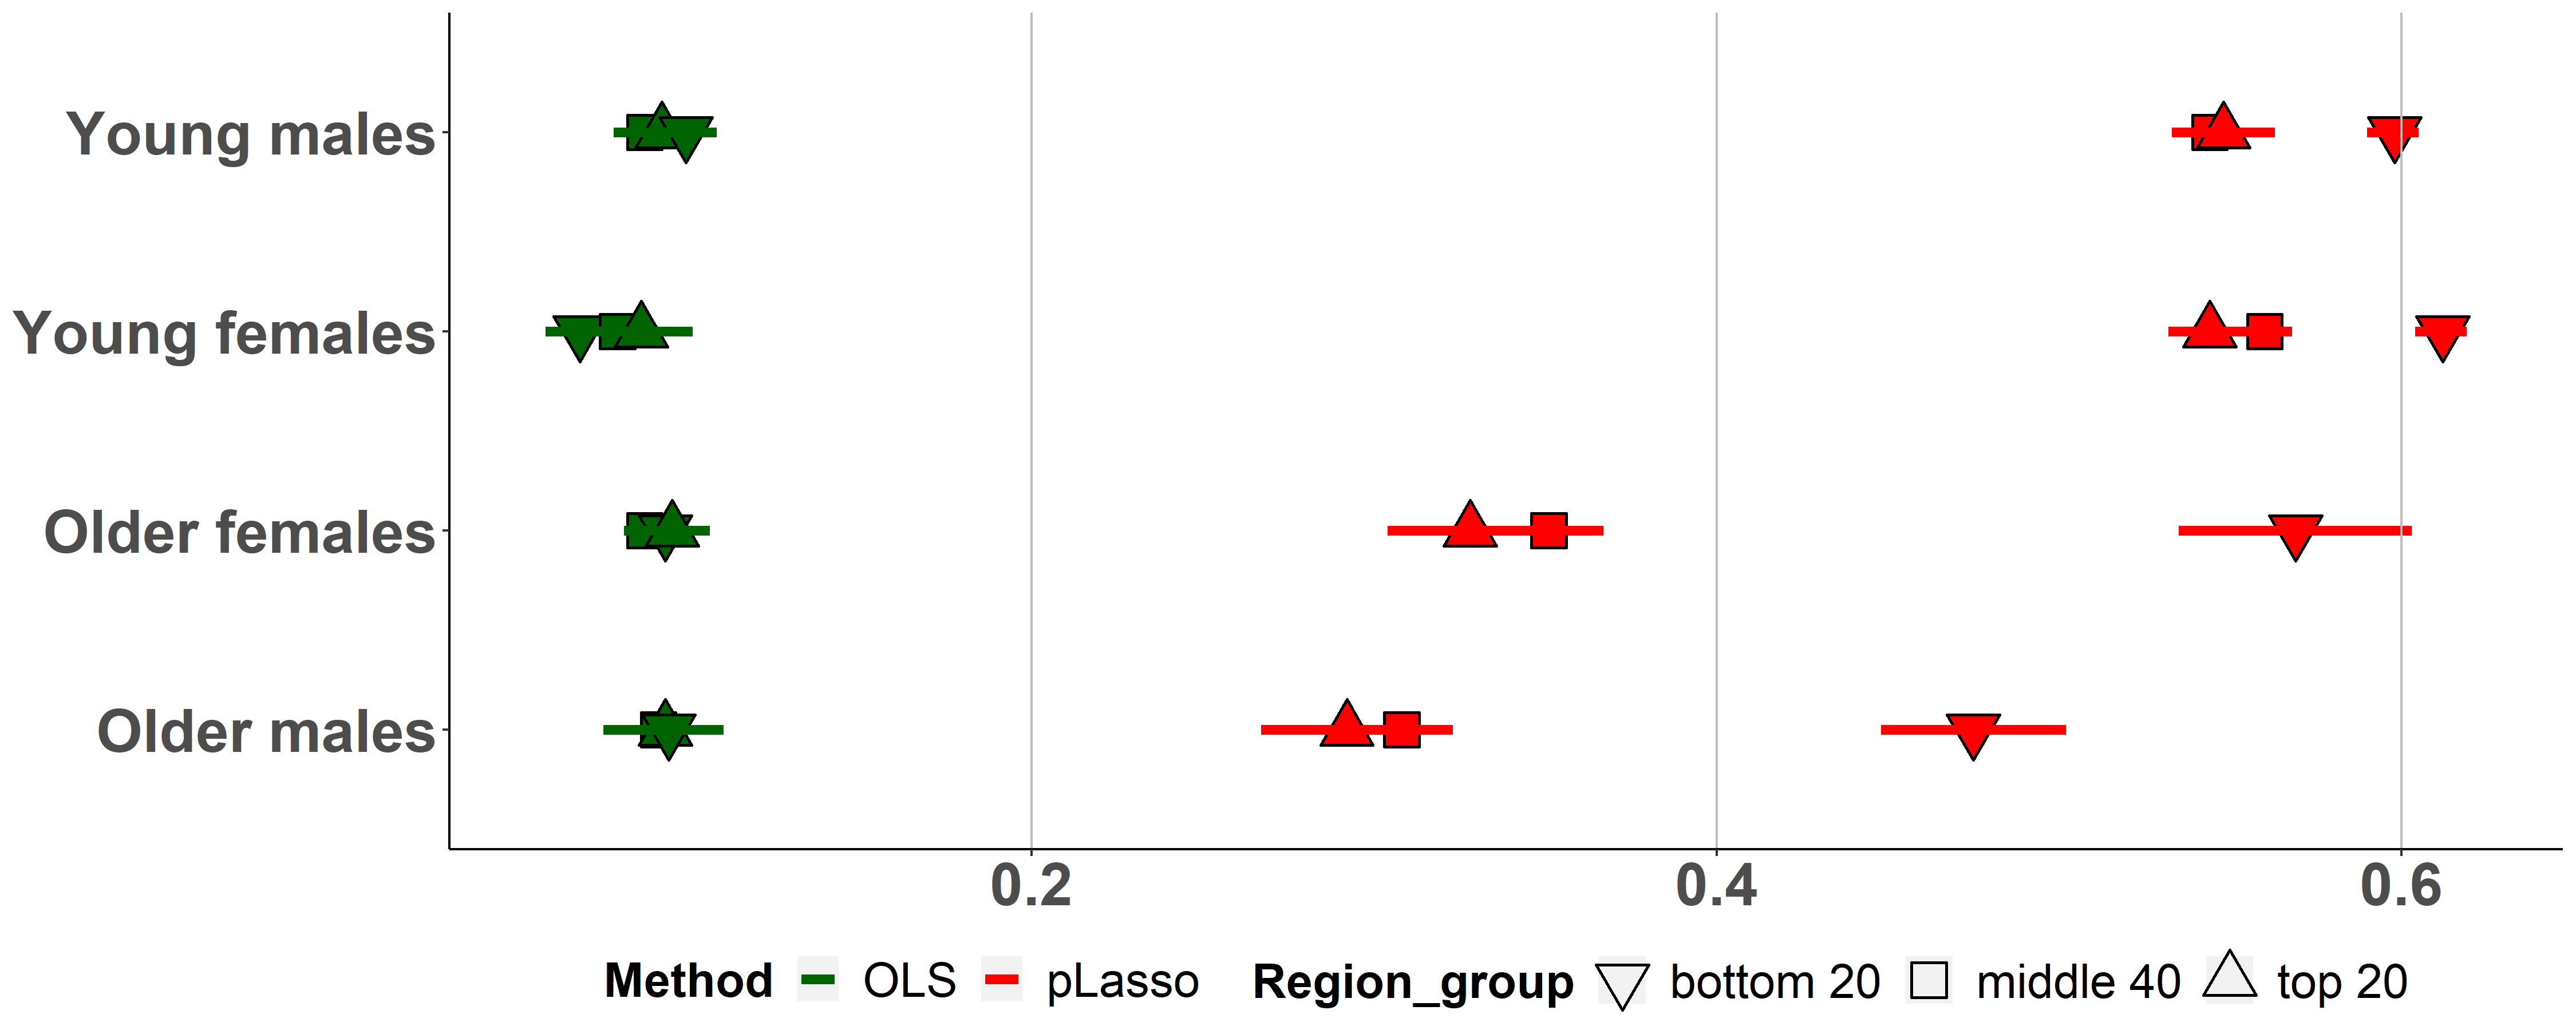
\includegraphics[width=\textwidth]{iv_2_methods_3.png}
		\subcaption{Ranking variable: regional employment level of vocational education holders multiplied with reciprocal of employment level of higher education holders}\label{fig:5.4c}
	\end{minipage}
	\caption{Returns to Education Estimates and 95\% CIs for Post-Lasso and OLS by Cohorts and Ranked Groups of Regions}
	\label{fig:5.4}
\end{figure}

\begin{figure}[H]
	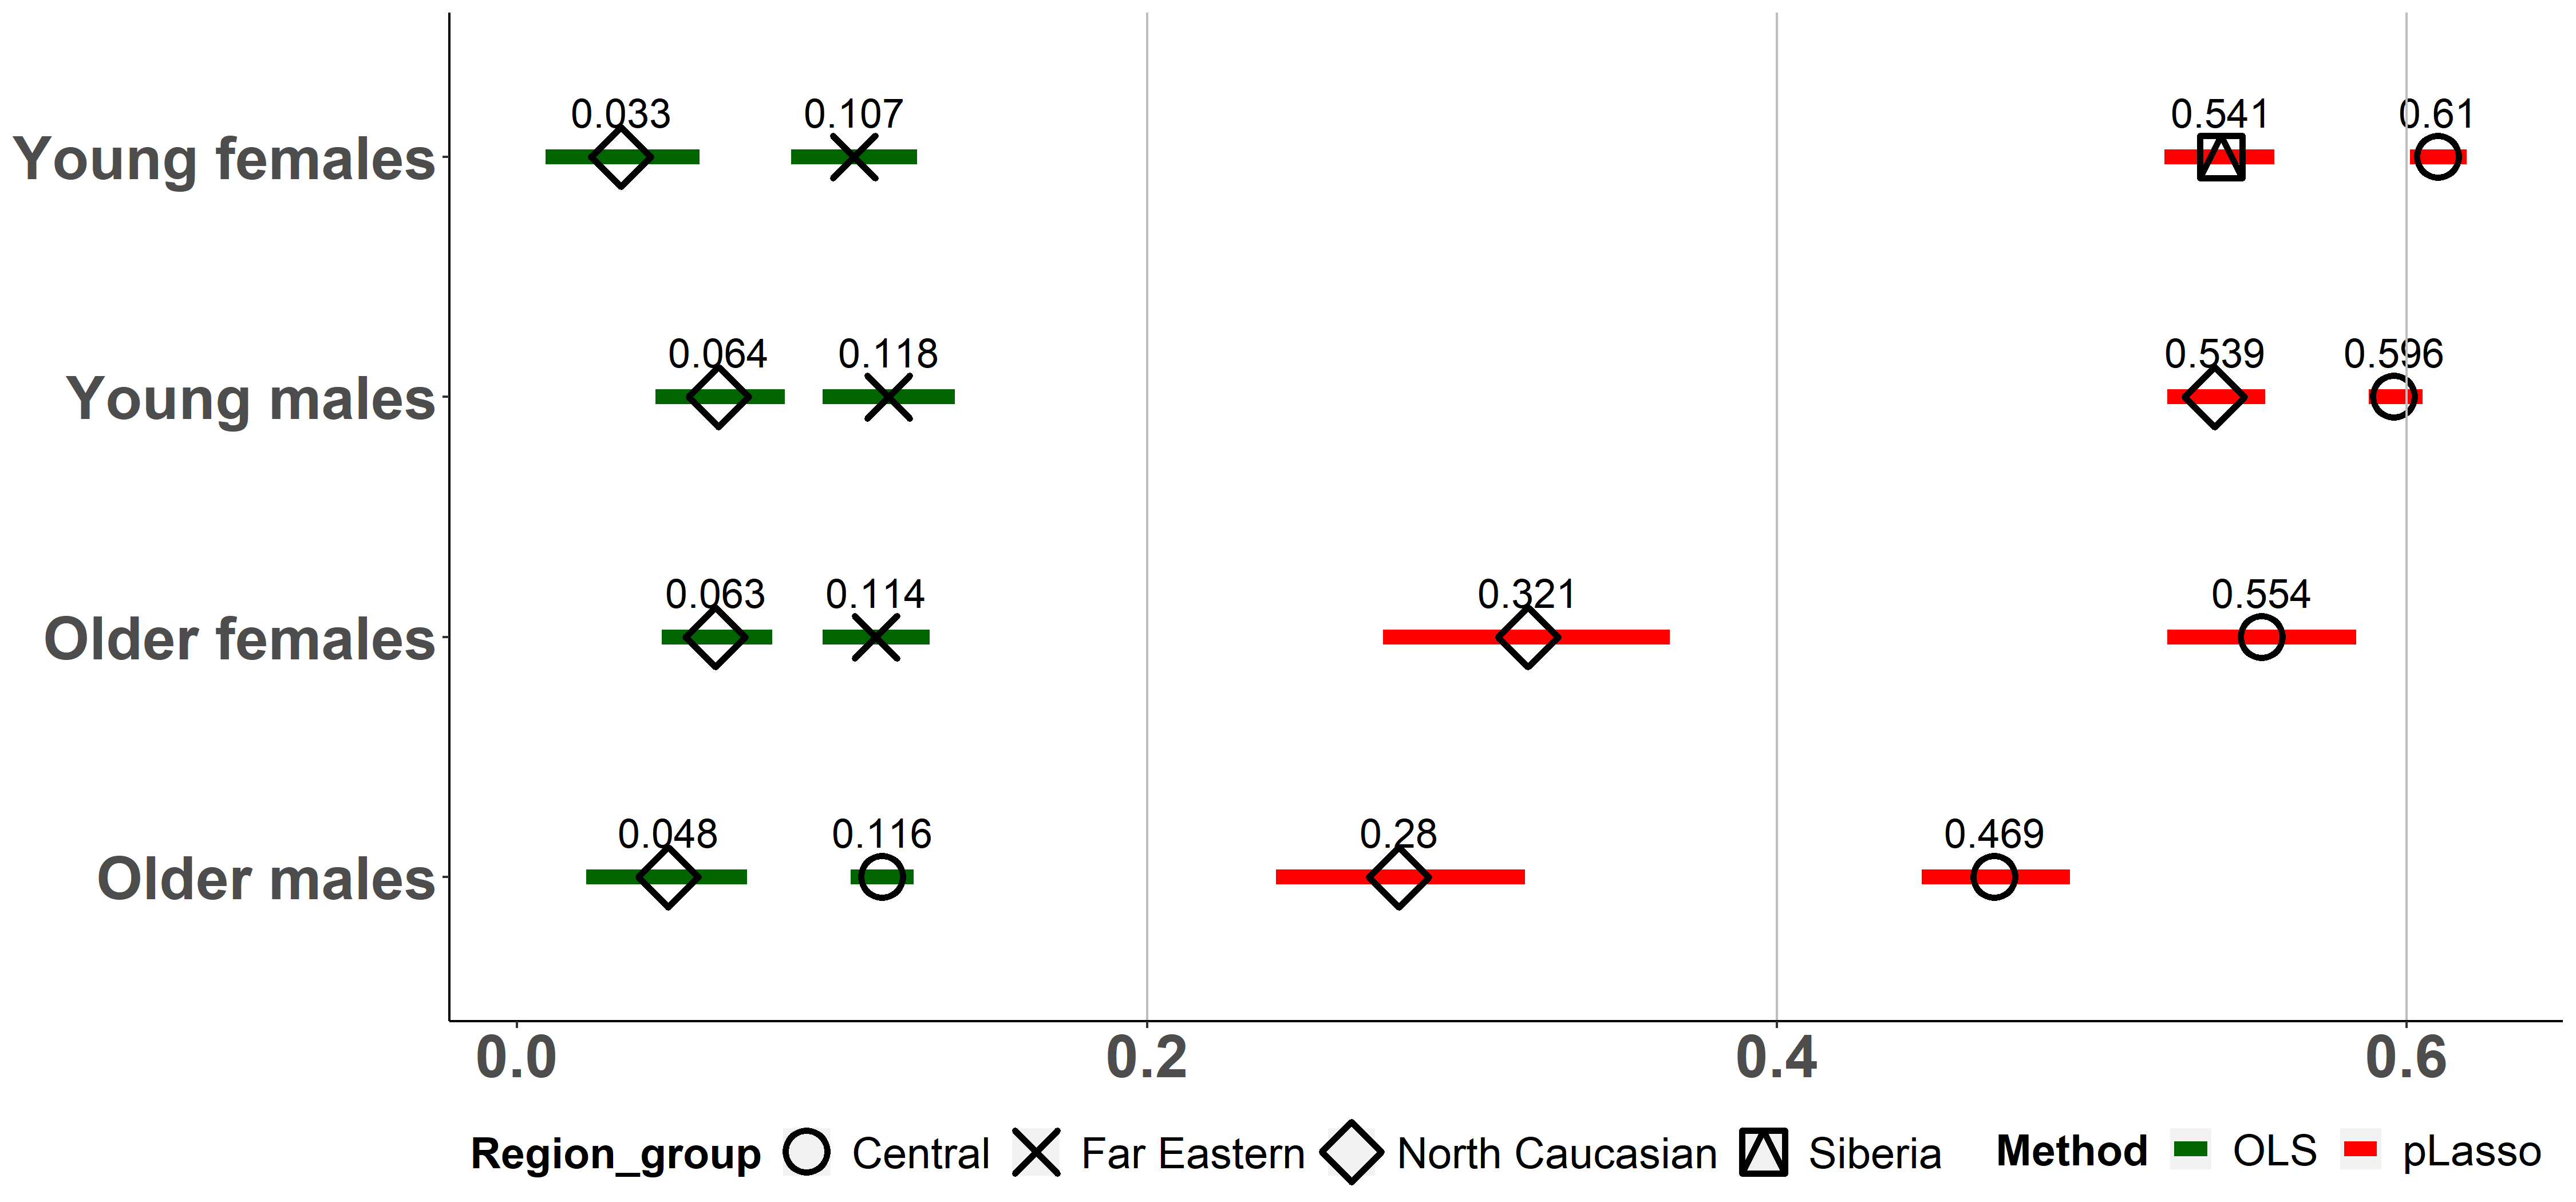
\includegraphics[width=\textwidth]{iv_by_districts.png}
	\caption{Returns to Education Estimates and 95\% CIs for Post-Lasso, 2SLS, and OLS by Cohorts} \label{fig:5.5}
\end{figure}


\begin{table}[ht]
	\centering
	\caption{Descriptive Statistics, RLMS}
	\label{tab:5.1}	
	\resizebox{\textwidth}{!}{
\begin{tabular}{lcccccccccc}
	\hline
	&  &  &  &  &  &  &  & \multicolumn{3}{c}{Education} \\ 
	&  & \multicolumn{2}{c}{Wage} & \multicolumn{2}{c}{Experience} & \multicolumn{2}{c}{Education years} & Secondary & Vocational & \multicolumn{1}{c}{Higher} \\ 
	Year  & N & Mean & SD & Mean & SD & Mean & SD & Percent & Percent & \multicolumn{1}{c}{Percent} \\ 
	\hline
	1994  & $3044$ & $\phantom{0}272761.9$ & $\phantom{0}347856.1$ & $\phantom{00000}21.4$ & $\phantom{000000}9.6$ & $\phantom{00000}12.7$ & $\phantom{000000}2.3$ & $\phantom{00000}22.3$ & $\phantom{00000}50.4$ & $\phantom{00000}27.3$ \\
	1995  & $2694$ & $\phantom{0}557844.7$ & $\phantom{0}621599.5$ & $\phantom{00000}21.7$ & $\phantom{000000}9.6$ & $\phantom{00000}12.7$ & $\phantom{000000}2.2$ & $\phantom{00000}22.3$ & $\phantom{00000}47.8$ & $\phantom{00000}29.8$ \\
	1996  & $2282$ & $\phantom{0}817936.7$ & $1004035.7$ & $\phantom{00000}21.6$ & $\phantom{000000}9.6$ & $\phantom{00000}12.8$ & $\phantom{000000}2.2$ & $\phantom{00000}19.7$ & $\phantom{00000}48.6$ & $\phantom{00000}31.7$ \\
	1998  & $3102$ & $\phantom{0000}906.3$ & $\phantom{0000}950.7$ & $\phantom{00000}22.3$ & $\phantom{000000}9.6$ & $\phantom{00000}12.7$ & $\phantom{000000}2.2$ & $\phantom{00000}19.8$ & $\phantom{00000}52.0$ & $\phantom{00000}28.2$ \\
	2000  & $3215$ & $\phantom{000}1821.3$ & $\phantom{000}2570.5$ & $\phantom{00000}22.3$ & $\phantom{00000}10.0$ & $\phantom{00000}12.7$ & $\phantom{000000}2.2$ & $\phantom{00000}20.3$ & $\phantom{00000}51.3$ & $\phantom{00000}28.4$ \\
	2001  & $3605$ & $\phantom{000}2681.0$ & $\phantom{000}2849.6$ & $\phantom{00000}22.0$ & $\phantom{000000}9.8$ & $\phantom{00000}12.8$ & $\phantom{000000}2.2$ & $\phantom{00000}19.8$ & $\phantom{00000}49.3$ & $\phantom{00000}30.9$ \\
	2002  & $3803$ & $\phantom{000}3612.8$ & $\phantom{000}4316.0$ & $\phantom{00000}22.0$ & $\phantom{000000}9.9$ & $\phantom{00000}12.8$ & $\phantom{000000}2.1$ & $\phantom{00000}19.3$ & $\phantom{00000}49.9$ & $\phantom{00000}30.8$ \\
	2003  & $3858$ & $\phantom{000}4378.6$ & $\phantom{000}4014.0$ & $\phantom{00000}22.2$ & $\phantom{00000}10.1$ & $\phantom{00000}12.8$ & $\phantom{000000}2.2$ & $\phantom{00000}19.1$ & $\phantom{00000}49.4$ & $\phantom{00000}31.5$ \\
	2004  & $3968$ & $\phantom{000}5379.0$ & $\phantom{000}4918.5$ & $\phantom{00000}22.0$ & $\phantom{00000}10.2$ & $\phantom{00000}12.8$ & $\phantom{000000}2.2$ & $\phantom{00000}18.4$ & $\phantom{00000}50.3$ & $\phantom{00000}31.2$ \\
	2005  & $3913$ & $\phantom{000}6637.9$ & $\phantom{000}5716.1$ & $\phantom{00000}22.1$ & $\phantom{00000}10.4$ & $\phantom{00000}12.8$ & $\phantom{000000}2.2$ & $\phantom{00000}18.4$ & $\phantom{00000}49.6$ & $\phantom{00000}32.0$ \\
	2006  & $4804$ & $\phantom{000}8089.9$ & $\phantom{000}6563.9$ & $\phantom{00000}22.2$ & $\phantom{00000}10.4$ & $\phantom{00000}12.8$ & $\phantom{000000}2.2$ & $\phantom{00000}18.0$ & $\phantom{00000}50.9$ & $\phantom{00000}31.1$ \\
	2007  & $4726$ & $\phantom{000}9662.5$ & $\phantom{000}7124.7$ & $\phantom{00000}22.5$ & $\phantom{00000}10.6$ & $\phantom{00000}12.8$ & $\phantom{000000}2.2$ & $\phantom{00000}18.5$ & $\phantom{00000}50.2$ & $\phantom{00000}31.3$ \\
	2008  & $4827$ & $\phantom{00}12826.3$ & $\phantom{00}10784.5$ & $\phantom{00000}22.6$ & $\phantom{00000}10.8$ & $\phantom{00000}12.9$ & $\phantom{000000}2.3$ & $\phantom{00000}17.9$ & $\phantom{00000}47.8$ & $\phantom{00000}34.3$ \\
	2009  & $4804$ & $\phantom{00}13363.1$ & $\phantom{00}10411.4$ & $\phantom{00000}22.5$ & $\phantom{00000}11.0$ & $\phantom{00000}12.9$ & $\phantom{000000}2.3$ & $\phantom{00000}16.6$ & $\phantom{00000}47.9$ & $\phantom{00000}35.5$ \\
	2010  & $7326$ & $\phantom{00}14769.9$ & $\phantom{00}12587.1$ & $\phantom{00000}22.6$ & $\phantom{00000}11.1$ & $\phantom{00000}13.0$ & $\phantom{000000}2.3$ & $\phantom{00000}16.9$ & $\phantom{00000}48.1$ & $\phantom{00000}34.9$ \\
	2011  & $7167$ & $\phantom{00}16226.8$ & $\phantom{00}12855.5$ & $\phantom{00000}22.5$ & $\phantom{00000}11.1$ & $\phantom{00000}13.0$ & $\phantom{000000}2.3$ & $\phantom{00000}18.0$ & $\phantom{00000}46.9$ & $\phantom{00000}35.1$ \\
	2012  & $7428$ & $\phantom{00}18880.7$ & $\phantom{00}15119.0$ & $\phantom{00000}22.5$ & $\phantom{00000}11.2$ & $\phantom{00000}13.0$ & $\phantom{000000}2.4$ & $\phantom{00000}18.2$ & $\phantom{00000}45.9$ & $\phantom{00000}35.9$ \\
	2013  & $7327$ & $\phantom{00}20601.4$ & $\phantom{00}16411.5$ & $\phantom{00000}22.5$ & $\phantom{00000}11.2$ & $\phantom{00000}13.1$ & $\phantom{000000}2.3$ & $\phantom{00000}17.0$ & $\phantom{00000}46.7$ & $\phantom{00000}36.3$ \\
	2014  & $6148$ & $\phantom{00}22772.6$ & $\phantom{00}17288.4$ & $\phantom{00000}22.3$ & $\phantom{00000}11.1$ & $\phantom{00000}13.1$ & $\phantom{000000}2.3$ & $\phantom{00000}16.5$ & $\phantom{00000}45.8$ & $\phantom{00000}37.7$ \\
	2015  & $6231$ & $\phantom{00}23570.7$ & $\phantom{00}16996.4$ & $\phantom{00000}22.2$ & $\phantom{00000}11.2$ & $\phantom{00000}13.2$ & $\phantom{000000}2.3$ & $\phantom{00000}15.2$ & $\phantom{00000}44.4$ & $\phantom{00000}40.4$ \\
	2016  & $6297$ & $\phantom{00}24951.1$ & $\phantom{00}18640.7$ & $\phantom{00000}22.3$ & $\phantom{00000}11.1$ & $\phantom{00000}13.3$ & $\phantom{000000}2.3$ & $\phantom{00000}14.7$ & $\phantom{00000}43.6$ & $\phantom{00000}41.8$ \\
	2017  & $6359$ & $\phantom{00}26254.1$ & $\phantom{00}19555.4$ & $\phantom{00000}22.4$ & $\phantom{00000}11.0$ & $\phantom{00000}13.3$ & $\phantom{000000}2.3$ & $\phantom{00000}14.0$ & $\phantom{00000}45.0$ & $\phantom{00000}40.9$ \\
	2018  & $6121$ & $\phantom{00}28081.0$ & $\phantom{00}19705.8$ & $\phantom{00000}22.5$ & $\phantom{00000}10.8$ & $\phantom{00000}13.3$ & $\phantom{000000}2.3$ & $\phantom{00000}13.8$ & $\phantom{00000}45.0$ & $\phantom{00000}41.2$ \\
	\hline 
\end{tabular}
}
\end{table}


\end{document}